\documentclass[12pt]{suhbook}
%% biber processes the reference db
%% citation keys and entries will be alphabetic
%% A reference section will be added to each chapter
\usepackage[demo]{graphicx}
\usepackage{titlesec}
\usepackage{subcaption}
\usepackage{siunitx}
\begin{document}
\setcounter{chapter}{3}% To jump to a chapter number, N-1 here
\chapter{Flexible Terahertz Antenna Design for Wearable Applications}
\section{Introduction}
Terahertz (THz) waves also known as sub-millimeter waves can be observed between the optical and microwave frequency regions of the electromagnetic spectrum \cite{liu2009advanced,grischkowsky1990far}. Devices operating in the optical and infrared spectra are generally characterized by beams containing many modes, and typically have dimensions much larger than the wavelength. On the contrary, THz frequency based devices are comparable in size to the operating wavelength \cite{shi2018thz}. Such devices have the potential to fulfil the future wireless communications needs of ultra-high bandwidths and date rates. Moreover, the problems of channel congestion can be overcome through the use of THz based communication systems. 
There has been an ever increasing demand of the data-based wireless communication in the past decade. Moreover, throughout the world urban population has been growing at an alarming rate. These two factors have created enormous challenges in implementing high-speed and reliable networks that can serve a large number of people at the same time \cite{song2011present}. A natural solution to overcome this challenge is to shift the network operating frequency to the THz region. However, with the available technologies, THz systems are affected by high atmospheric attenuation, and much lower propagation distances which demand for novel techniques through which the performance of a THz based communication system can be increased. To do so, micro and nano scale device fabrication techniques have been actively studied of late. Additionally, the search for highly conductive materials is an active research area to develop  efficient THz devices.

In conventional wireless communication systems, metallic antennas are fabricated separately from the microelectronics. It is not currently possible to operate circuitry in the THz frequency region simply by down-scaling the traditional metallic antenna to a few micrometres \cite{kleine2011review}. By moving up in the frequency, the device physics changes drastically and the approach of using a metal based antenna has several limitations, chief among them is the low mobility of electrons in the nano-scale metallic structures. This results in the antennas being highly lossy at the resonant frequencies, which would result in high attenuation and subesequently poor efficiency of the system \cite{pourahmadazar2018millimeter}. To address this lossy behaviour, meta-material based nano-structures have emerged as attractive solutions. \cite{chen2006active}.
% 
% 
% 
\section{Terahertz Antenna Designs}
% 
\subsection{Graphene based Terahertz Antenna}
% 
Graphene is an atomically thin, two-dimensional crystalline form of carbon in which the carbon atoms are arranged in the form of a hexagonal lattice structure. It was discovered in 2004 by Novoselov and Geim, who peeled off a small amount of monolayer graphene with the help of an adhesive tape, therefore, obtaining free-standing graphene in air \cite{novoselov2004electric}. For their ground-breaking discovery, they were awarded the Nobel Prize in Physics in 2010. Graphene is considered one of the thinnest and in terms of mechanical properties, the strongest material measured  \cite{campos2008bulk,lee2013high}. Its theoretical specific surface area is as high as \SI{2630}{\square\m\per\gram}, thermal conductivity as high as \SI{5300}{\watt \per \m \per \kelvin}, which is higher than that of carbon nano-tube and diamond. In terms of electromagnetic properties, it is almost completely transparent, absorbing only 2.3\% of light. On the other hand, graphene also has a very high electron mobility of \SI{15000}{\square\cm \per\volt\per\siemens} at room temperature, which is higher than that of carbon nanotube or crystalline silicon \cite{ju2011graphene}. Nonetheless, the electrical resistivity of graphene is of the order of $10^{-6}\Omega \cm$ ower than copper and silver, which are the best conducting materials. All these attractive characteristics enable graphene to display extra-ordinary electromagnetic phenomena. When an electromagnetic wave is obliquely incident wave upon graphene, surface plasmon polaritons (SPPs) are excited. Due to the high conductivity of graphene, the SPPs are tightly confined to the graphene surface having wavelength much smaller than its free-space equivalent. Moreover, the graphene SPPs exhibit  moderate loss, and a vital property of tuning the resonant frequency through external electrical and magnetic bias, and chemical doping. Most importantly, the resonant frequency of graphene lies in the THz and mid-infrared frequency ranges. The likelihood of creating lightweight, dainty and minimal effort adaptable antenna gadgets imperative preferred standpoint of utilizing graphene material. Joined with other significant favorable position in lightweight, mechanical adaptability, printed graphene can be bargain creation minimal effort consumable wearable antenna.
Using a semi-classical electronic model in the absence of magnetic bias, graphene’s conductivity can be expressed at THz frequencies by using the interband term of the Kubo formula \cite{tamagnone2012analysis},
% 
\begin{equation} 
\sigma \left( \omega \right) \approx -j \frac{{e}^{2} k_{B} T}{\pi \hbar^{2}(\omega - j \tau^{-1})}  \times\left(\frac{\mu_{c}}{k_{B} T} + 2 \ln \left(e^{-\mu_{c} /\left(k_{B} T\right)}+1\right)\right) 
\label{eq:conductivity}
\end{equation}
Where \si{e} is the electron charge,\si{\tau} is the electron relaxation time in graphene,\si{k_B}is the Boltzmann’s constant,\si{T} is temperature,\si{\hbar} is the reduced Planck’s constant, \si{\omega} is the angular frequency, and \si{\mu_c} graphene’s chemical potential. The interband transitions (imaginary part in \eqref{eq:conductivity}) only occur when $\hbar\omega < 2\mu_c$, which is true in the case of operating at THz frequencies for moderate \si{\mu_c}. For graphene, one of the most significant characteristics is the ability to control or in other words, tune the complex-valued conductivity. This can be done by exploiting the field effect field effect with an application of an external electrostatic field bias. The opto-electronic response of graphene described by the parameters such as the chemical potential \si{\mu_c} and relaxation time \si{\tau} can therefore be computed through be calculated by equations \cite{abadal2015time}. 
\begin{equation}
\mu_c=\hbar V_f\sqrt{\pi n}
\label{eq:chemical}
\end{equation}

\begin{equation}
\tau=\frac{\mu_c\mu}{e V^2_f}
\label{eq:relax time}
\end{equation}
\si{V_f} fermi velocity $(10^6 s\backslash m)$, \si{\mu_c} the chemical potential, \si{e} is the elementary charge,\si{\mu} is the carrier mobility of the electrons and \si{n} is the carrier density. Graphene conductivity strongly depends on the chemical potential and the relaxation time, in very low chemical potential and carrier mobility conditions, relatively invalid drive reactions are gotten. This infers that reverberation is not accomplished because of the attenuation of SPP waves as they propagate on the surface of the graphene. In request to acquire a non-irrelevant resonant conduct, such impacts must be diminished by methods for enhancing either the chemical potential or the carrier mobility, the relaxation time of the material and leads to a stronger radiated field. 
Although both the increase of the chemical potential and the carrier mobility contribute to a raise of the radiated energy, the impact on the impulse response is different in each case, However, the increase in radiated energy affects the width of the response and the ringing tail rather than the pulse amplitude. Such broadening of the temporal response is coherent with the sharpening of the resonant behaviour that is observed when the carrier mobility is improved. A stronger resonant behaviour is observed as the relaxation time is increased, value of the relaxation time \si{\tau} has a huge impact on the resonant character of the graphene and its bandwidth.
\subsection{Graphene Antenna for Wearable Applications}
Graphene antenna was designed utilizing CST microwave studio \si{2018}, at the temperature of \SI{293}{\kelvin}. The patch antenna consisting of a graphene patch, ground plane, and dielectric substrate, the antenna design shown in figure \ref{Fig 1}.The ground plane and transmission feed line made of graphene material to enhance the flexibility and fitness of the antenna to different fabrication techniques. In terms of chemical potential, this paper examines the antenna in the range of chemical potential between \SI{0.1}{e \volt} to \SI{0.4}{e \volt} and relaxation time between \SI{0.1}{\pico \second } to \SI{0.8}{\pico \second }. Figure \ref{Fig 2} shows the resonant frequencies of the proposed antenna. As the relaxation time continues to increase, higher order resonances appear, and an intense resonant behavior is noted.
\begin{figure}[hbt!]
    \centering
    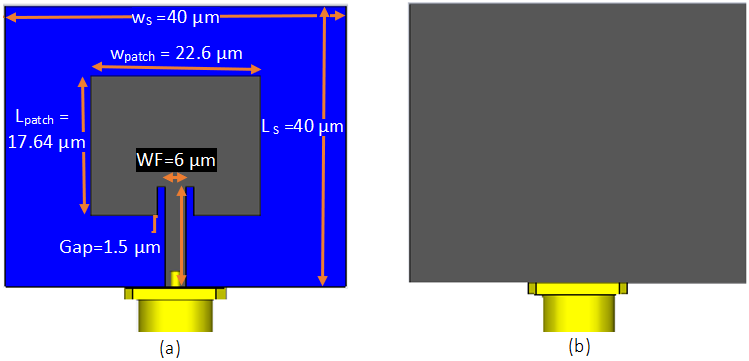
\includegraphics[width=0.6\textwidth]{1}
    \caption{Flexible terahertz graphene antenna design}
    \label{Fig 1}
\end{figure}
\begin{figure}[h]
    \centering
    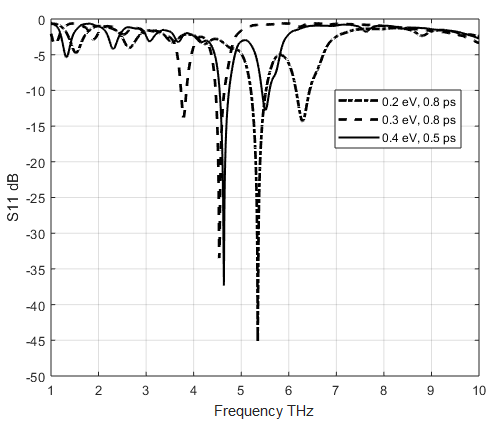
\includegraphics[width=0.6\textwidth]{2}
    \caption{Reflection coefficient (\si{S_{11}}) at range of chemical potential and relaxation time (black 0.2 eV, blue 0.3 eV and brown 0.4 eV), relaxation time from 0.1 to 0.8 ps}
    \label{Fig 2}
\end{figure}
\\The greatest value of the reflection coefficient (\si{S_{11}}) is \SI{-45}{\deci\bel} obtained at \SI{0.4}{e \volt} chemical potential and \SI{0.5}{\pico \second } relaxation time. The resonant frequency of the graphene also changes when varying the chemical potential as shown in figure \ref{Fig 2}, at \SI{0.4}{e \volt} the resonant frequency changed to \SI{4.636}{\THz} instead of \SI{4.546}{\THz} at \SI{0.2}{e \volt} and the \si{S_{11}} started to increase from\SI{-34}{\deci\bel} to almost \SI{-37}{\deci\bel} . At \SI{0.4}{e \volt}, \si{S_{11}} still below \SI{-10}{\deci\bel} at \SI{0.1}{\pico \second } relaxation time, to get greater reflection coefficient, relaxation time must be increased, as result \si{S_{11}}increased to \SI{-45}{\deci\bel} when relaxation time reaches \SI{0.5}{\pico \second }, the resonant frequency shifted to \SI{5.3}{\THz} as an alternative of \SI{4.7}{\THz} at \SI{0.3}{e \volt}. The antenna has three possible resonant frequencies as shown in \ref{table:1}.The thickness of the substrate is evaluated to optimize the antenna performance in terms of the reflection coefficient and bandwidth. From figure \ref{Fig 3}, the substrate thicknesses obviously affect the \si{S_{11}} value, however, the bandwidth becomes narrower with increasing substrate thickness (Table \ref{table:2}).
\begin{table}[hbt!]
\centering
 \begin{tabular}[hbt!]{||c c c c||} 
 \hline
 Frequency & Chemical Potential & Relaxation time & Bandwidth \\ [0.5ex] 
 \hline\hline
 4.546 THz & 0.2 eV & 0.8 ps & 185 GHz \\ 
 \hline
 4.636 THz & 0.3 eV & 0.8 ps & 204 GHz \\
 \hline
 5.347 THz & 0.4 eV & 0.5 ps & 310 GHz \\[1ex] 
 \hline
\end{tabular}
\caption{The effect of chemical potential and relation time on resonant frequency and bandwidth}
\label{table:1}
\end{table}
\begin{figure}[hbt!]
    \centering
    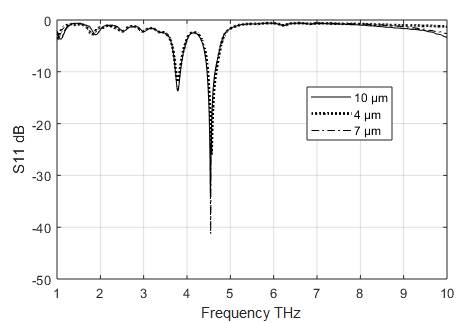
\includegraphics[width=0.5\textwidth]{3}
    \caption{Substrate thickness (red 7 micrometers, green 10 micrometers, blue 4 thickness)}
    \label{Fig 3}
\end{figure}
\begin{table}[hbt!]
\centering
 \begin{tabular}{||c c c c||} 
 \hline
Substrate Thickness & Frequency & Bandwidth & Reflection coefficient (\si{S_{11}}) \\ [0.5ex] 
 \hline\hline
\SI{4}{\mu_m} & 4.546 THz & 193.9 GHz & 26 dB \\ 
 \hline
\SI{7}{\mu_m} & 4.546 THz & 192 GHz & -41 dB  \\
 \hline
 \SI{10}{\mu_m} & 4.546 THz & 185 GHz & -33.3 dB \\[1ex] 
 \hline
\end{tabular}
\caption{The effect of substrate thickness on the reflection coefficient value and bandwidth }
\label{table:2}
\end{table}
\\As a result, the \SI{7}{\mu_m} substrate thickness has the greater negative \si{S_{11}} of \SI{-41}{\deci\bel}and bandwidth of \SI{192}{\GHz}. Obviously choosing of specific substrate thickness is a critical choice, the substrate thickness has an influence on the performance of the antenna designing.The flexible substrate material is important for the wearable application, to compare different types of flexible substrate material, \SI{0.2}{e \volt} chemical potential, and \SI{0.8}{\pico \second } relaxation time values are selected.From figure \ref{Fig 4}, polyamide substrate appears to give the largest negative \si{S_{11}} of \SI{-42}{\deci\bel}. Polyimide substrate is appropriate for applications demanding a high degree of dimensional stability after the experience to extreme temperatures. Moreover, polyimide offers a high flexibility and low profile making it the perfect substrate material for printed fabrication techniques. The Rogers \si{3006} substrate materials achieved\SI{-40.6}{\deci\bel} , and Polyethylene terephthalate (PET) \SI{-30}{\deci\bel}, paper below \SI{-30}{\deci\bel}. Based on \SI{7}{\mu_m}  substrate thickness, different resonant frequencies can be achieved by means of doping and external biasing figure \ref{Fig 5}.Table \ref{table:3} breakdown a comparison between the three different resonant frequencies at \SI{7}{\mu_m} substrate thickness. All the frequencies have approximately the same\si{S_{11}} with the difference in bandwidth which increases with higher chemical potential value. As the chemical potential goes higher, the bandwidth increased. On the other hand, the transmission range became lesser when the electric potential is increased, and the more is the absorption energy and resonant energy which will reduce their transmission range. High main lobe magnitudes and lower side lobe levels can be observed from figure \ref{FIG 6} and \ref{FIG 7}. the main lobe magnitude in E-plane started at \SI{2.93}{\deci\bel} at \SI{0.2}{e \volt} chemical potential, at the higher chemical potential it became lesser,\SI{1.51}{\deci\bel} at \SI{0.3}{e \volt}and \SI{-1.41}{\deci\bel} at \SI{0.4}{e \volt}.The proposed antenna has proved the tenability of graphene antenna to resonate at different frequencies in terahertz band, \SI{4.546}{\THz}, \SI{4.636}{\THz} and \SI{5.347}{\THz} by varying the chemical potential and relaxation time. Varying the chemical potential lead to increase the bandwidth from \SI{199}{\GHz} at\SI{0.2}{e \volt} to \SI{314}{\GHz} at \SI{0.4}{e \volt}. On the other hand, chemical potential has affected the radiation pattern by increasing the side lobe and reducing the directivity of the proposed antenna. Analysis has also been performed to evaluate the antenna bandwidth and reflection coefficient (\si{S_{11}}) at resonant frequencies. A comparison between different flexible substrate allows us to evaluate the effect of substrate material on the antenna performance, graphene antenna with polyamide substrate shows the maximum\si{S_{11}} of \SI{-42}{\deci\bel} . Flexibility and unique performance of designed antenna recommended for wearable applications.
\begin{figure}[hbt!]
\centering
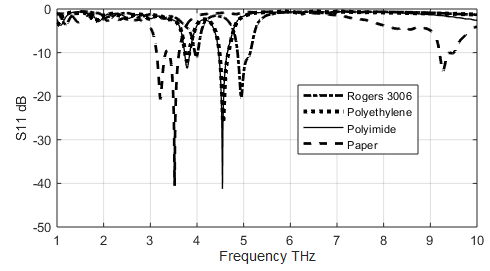
\includegraphics[width=0.5\textwidth]{4}
\caption{Reflection coefficient (\si{S_{11}}) of different substrate material thickness \SI{7}{\mu_m},black Rogers 3006, blue Polyethylene, green polyimide, brown paper.}
\label{Fig 4}
\end{figure}
\begin{figure}[h]
\centering
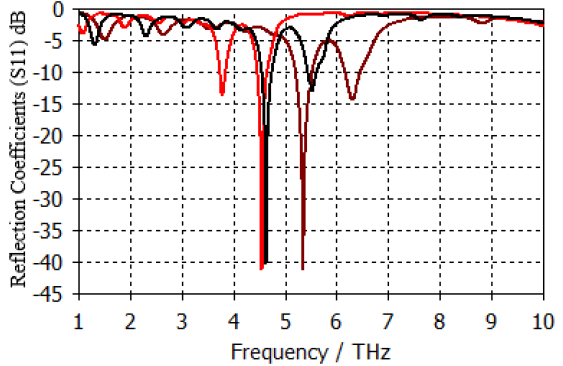
\includegraphics[width=0.5\textwidth]{5}
\caption{Antenna resonant frequencies at \SI{7}{\mu_m} thickness(0.2 eV and 0.8 ps red, 0.3 eV and 0.8 ps,black 0.4 eV and 0.5 ps)}
\label{Fig 5}
\end{figure}
\begin{table}[hbt!]
\centering
\begin{tabular}{||c c c c c||}
\hline
Frequency & Chemical Potential & Relaxation time & Reflection Coefficient (\si{S_{11}}) & Bandwidth \\[0.5ex] 
\hline\hline
4.546 THz & 0.2 eV & 0.8 ps &  -41.258 dB & 199 GHz \\ 
\hline
4.636 THz & 0.3 eV & 0.8 ps & -40.187 dB & 279.9 GHz \\
\hline
5.347 THz & 0.4 eV & 0.5 ps & -41.283 dB & 314 GHz \\[1ex] 
\hline
\end{tabular}
\caption{A comparison between different resonant frequencies at \SI{7}{\mu_m} substrate thickness }
\label{table:3}
\end{table}
\begin{figure}[hbt!]
\begin{subfigure}{.5\textwidth}
  \centering
  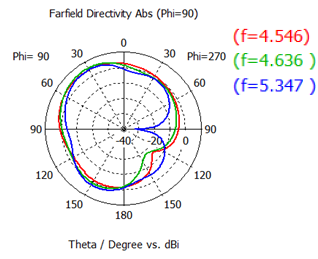
\includegraphics[width=.9\linewidth]{6}
  \caption{H-plane}
  \label{FIG 6}
\end{subfigure}%
\begin{subfigure}{.5\textwidth}
  \centering
  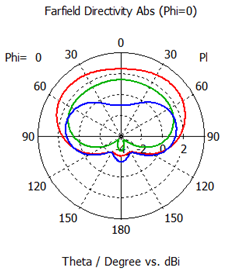
\includegraphics[width=.8\linewidth]{7}
  \caption{E-plane}
  \label{FIG 7}
\end{subfigure}
\caption{Simulations of the normalized field patterns in the E plane and H plane [ 4.546 THz red, 4.636 THz green, 5.347 THz blue]}
\label{fig:fig}
\end{figure}
\newpage
\subsection{The Effect of Human Body on the antenna radiation characteristics}
The demand for wearable devices is expected to increase to  \si{187.2}  million wearable units annually by \si{2022} \cite{hernandez2019wearable}. Wearable antenna requirements for all modern applications require lightweight, low cost, and a flexible profile. For wireless body area network (WBAN) scenarios, the antenna design becomes more complicated than simple free space environments, due to the absorption of the human skin. Human skin is a complex heterogeneous and anisotropic medium, where the small parts, like blood vessel and pigment content are spatially distributed in depth \cite{flynn2011modeling}. With the complexity of human skin, it is challenging to accurately describe the system, mainly due to the shapes and functions, and most importantly because of the absence of the dielectric constant measurements at high frequency \cite{alekseev2007human}. Therefore, most of the latest research simulate the human skin using \si{3} layers of epidermis, dermis, and hypodermis which represent the most essential parts of the human skin \cite{lynch1989growth}. As wearable antennas work close to the human body, the antenna performance will be affected as a consequence, due to absorption of the radiated energy. Therefore, wearable antennas should be carefully designed to achieve all the important properties of antenna whether they work close to the human body or inside the human body. Graphene conductivity strongly depends on the chemical potential and relaxation time. In addition, frequency shifting, and a wider bandwidth can be achieved by increasing the chemical potential and cross bounding relaxation time. On the other hand, increasing chemical potential has an impact on the radiation efficiency due to the growth of absorption level in graphene. Consequently, the reflection coefficient (\si{S_{11}}) will show a good matching between the source and the feed line but the radiation efficiency will decline as more power will be absorbed in the graphene material and causes loss of power. For simplicity, the typical value of chemical potential \SI{0}{e \volt} and relaxation time \SI{0.1}{\pico \second } has been chosen in order to obtain sufficient radiation and total efficiency and minimises the absorption in the material.
\begin{figure}[hbt!]
\centering
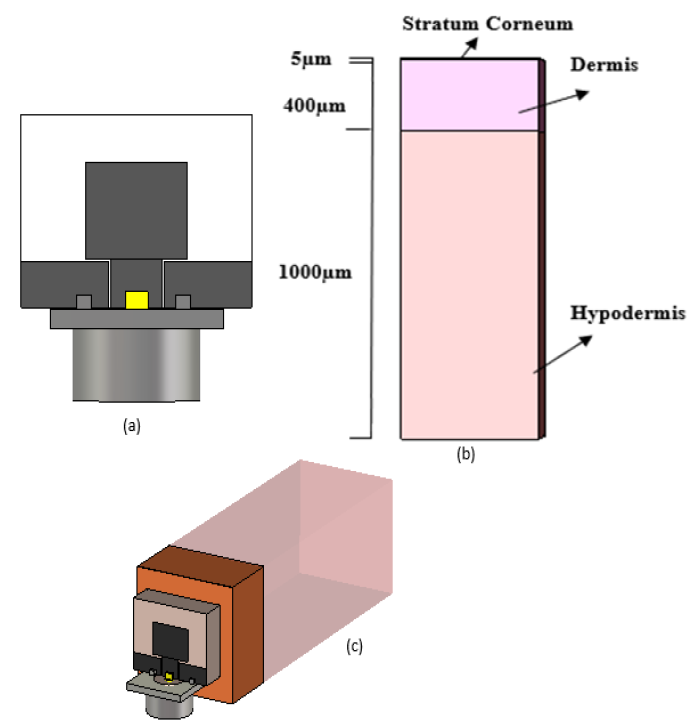
\includegraphics[width=0.6\textwidth]{8}
\caption{Geometry of the proposed patch antenna (a) Front view and (b) Human skin model (c) side view of the antenna on the human body}
\label{Fig 8}
\end{figure}
\\Figure \ref{Fig 8}a shows the geometry and parameters of the proposed CPW fed antenna. The proposed antenna is designed using CST Microwave Studio \si{2018}. The designed graphene-based antenna is tested in simulation at the room temperature of \SI{293}{\kelvin}. The antenna design with dimensions of \SI{260}{\mu_m} \times \SI{195}{\mu_m} \times \SI{0.35\times2}{nm} two layers of graphene, consisting of a graphene-based rectangular patch with feedline \SI{120}{\mu_m} \times \SI{100}{\mu_m} \times \SI{0.35\times2}{nm} made from graphene. The substrate material supervises the variation in radiation qualities of the graphene antenna. Rogers \si{3006} is used as substrate with thickness of \SI{175}{\mu_m} (dielectric constant,$\varepsilon_r = 6.5$, loss tangent, $\tan {\alpha} = 0.002$. Three layers of human skin model as shown in \ref{Fig 8}b, the thickness of which differ between various human skins. For the epidermis, the typical thickness ranges from \si{0.05} to \SI{1.5}{mm}, \SI{1.5-4}{mm} for the dermis, the hypodermis has no typical value \cite{dashti2018graphene}. The epidermis contains two layers, stratum corneum with only dead squamous cells and the living epidermis layer, where most of the skin pigmentation stay.\cite{abadal2015time}. The stratum corneum is a thin accumulation on the skin outer surface. The dermis, that supports the epidermis, is thicker and mainly composed of collagen fibers and intertwined elastic fibers enmeshed in a gellike matrix. The subcutaneous fat layer is composed of the packed cells with considerable fat, where the boundary is not well defined, thus, the thickness of this layer differs widely for various part of the human body. The permittivity of the human skin tissues can be obtained using,\cite{berry2003optical} \cite{yang2015numerical}.
\begin{equation}
   \epsilon^- =n^2-e^2
   \label{eq:real perimttivity}
\end{equation}
\begin{equation}
\epsilon^= =2nk
\label{eq:imag perimttivity}
\end{equation}
where $\epsilon^-$ and $\epsilon^=$ are respectively, the real and imaginary parts of the permittivity of the tissues,\si{n} is the refractive index, and \si{k} is the extinction coefficient. The refractive index is \si{1.97}, \si{1.73} and \si{1.58} for blood, skin, and fat, respectively \cite{yang2015numerical}. The extinction coefficient is calculated using the measured absorption coefficient data available in \cite{fitzgerald2003catalogue} \cite{berry2003optical} through,
\begin{equation}
k=\frac{\alpha\lambda_0}{4\pi}
\label{eq:abdorption}
\end{equation}
\\where $\lambda_0 = c/f$ is the wavelength in free-space, and $\alpha$  absorption coefficient.Figure \ref{Fig 8AE} demonstrates the scattering parameter (\si{S_{11}}) in free space. It has been observed that resonant frequency can be shifted towards lower range with the increase in length patch from \SI{195}{\mu_m} to\SI{215}{\mu_m}. The \si{S_{11}} of the graphene patch antenna is \SI{-46}{\deci\bel} at \SI{0.647}{\THz} obtained with length of \SI{195}{\nu_m}. The antenna gives a wide bandwidth \SI{29.2}{\GHz} which is the main advantage of this high frequency at wearable applications. Various parameters such as gain, reflection coefficient, efficiency, and radiation pattern of the proposed antenna are compared under free space and on body conditions. From figure \ref{Fig 8B}, the reflection coefficient of the patch antenna in the on-body state is shifted slightly towards the right side of the \SI{0.6482}{\THz} resonant frequency.\\
\begin{figure}[hbt!]
    \centering
    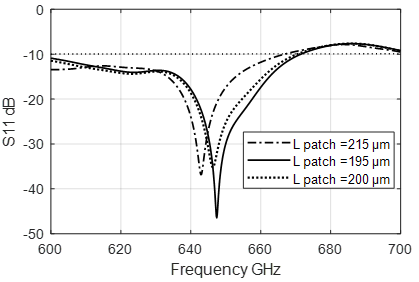
\includegraphics[width=0.6\textwidth]{9}
    \caption{\si{S_{11}} of the antenna with different patch length}
    \label{Fig 8AE}
\end{figure}
\begin{figure}[hbt!]
    \centering
    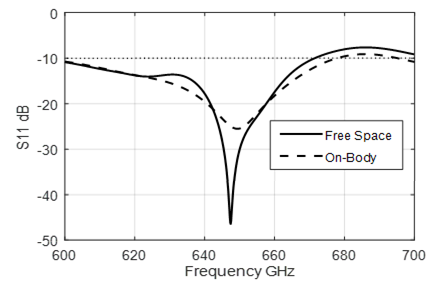
\includegraphics[width=0.6\textwidth]{10}
    \caption{\si{S_{11}} at On-body and free space.}
    \label{Fig 8B}
\end{figure}
\begin{figure}[hbt!]
    \centering
    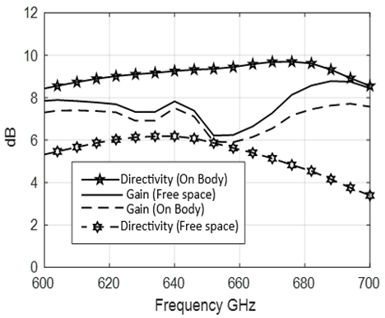
\includegraphics[width=0.6\textwidth]{11}
    \caption{Simulation gain and directivity on free space and on Body}
    \label{Fig 8AA}
\end{figure}
\begin{figure}[hbt!]
    \centering
    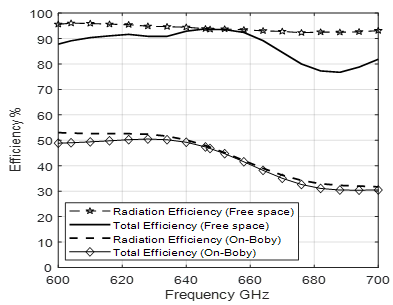
\includegraphics[width=0.55\textwidth]{12}
    \caption{Radiation and total efficiency on Free space and on Body}
    \label{Fig 91}
\end{figure}
\begin{figure}[hbt!]
\begin{subfigure}{.5\textwidth}
\centering
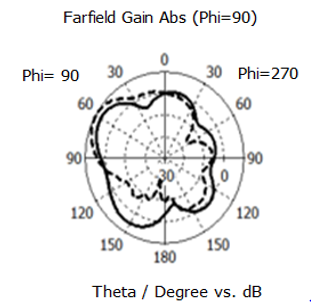
\includegraphics[width=.9\linewidth]{13}
\caption{H plane}
\label{fig:sfig10a}
\end{subfigure}%
\begin{subfigure}{.6\textwidth}
  \centering
  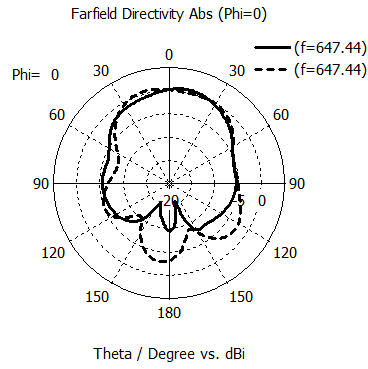
\includegraphics[width=.9\linewidth]{14}
  \caption{E plane}
  \label{fig:sfig2}
\end{subfigure}
\caption{The Hand E-plane radiation patterns of the graphene patch antenna and on and space}
\label{fig 14b}
\end{figure}
The \si{S_{11}} parameter of the graphene patch antenna on the body is \SI{-25}{\deci\bel}. The detuning of frequency is due to the high dielectric constant property of three layers of the human body. Because of these properties of the human body, most of the radiated waves propagate through the body and dissipate in the form of heat resulting in a wider\SI{-10}{\deci\bel} bandwidth. Due to the body absorption, the antenna gains decrease from \SI{-7.8}{\deci\bel}  to \SI{-7.2}{\deci\bel}. The gain of the antenna is a figure of merit of how well the antenna converts delivered power into radiated waves toward a specified direction.The decrease of the gain in the on body state is accompanied with an increase in the directivity. It is clear from figure \ref{Fig 8AA}  that for the antenna in the on body case, the value of gain at \SI{0.647}{\THz} decreases by \SI{0.3}{\deci\bel}, while the directivity increased by \SI{3}{\deci\bel}. The lower gain value obtained due to a decrease in the radiation efficiency, down from 96\% to almost 50\% (Figure \ref{Fig 91}). Therefore, the total radiated efficiency of antenna on flat body phantom decreases by (46\%). This is due to the higher conductivity of the outer most layer skin. The antenna total efficiency in the presence of the human body also decreases due to absorption in the lossy human body tissues. 
\\The H and E plane radiation patterns of the graphene patch antenna on the body and free space are shown in figure \ref{fig 14b}. The radiation pattern of both states is adequately consistent at the desired resonant frequency. The main lobe with \SI{-6.87}{\deci\bel} is obtained at the resonance of \SI{0.647}{\THz}, while an increase in the magnitude of the main lobe is observed at on body state with \SI{9.7}{\deci\bel}. Similarly, the side lobe in the on body case is \SI{-8 }{\deci\bel} and on free space is \SI{-2 }{\deci\bel}  due to higher reflections from the body surface. A wearable graphene THz antenna is presented and tested on three layers of human skin to serve the wearable applications in modern THz systems to achieve high performance. The results show that the designed antenna presented at\SI{0.647}{\THz}, have a realized gain of \SI{7.8 }{\deci\bel} and \SI{7.2 }{\deci\bel} on free space and on-body cases respectively. The radiation efficiency dropped from 96\% to 50\% when placed on body. We believe that the antenna will perform well when positioned at a distance of \si{1} or 2\mm from the human body surface. The antenna is regarded as a potential candidate for the future short-range wireless body area network (WBAN) Scenario.
\subsection{Perovskite material}
The expressions perovskite and perovskite structure are regularly utilized conversely. In fact, a perovskite is a sort of mineral that was first discovered in the Ural Mountains and named after Lev Perovskite (Russian scientist)\cite{park2016organic}. A perovskite structure is any intensify that has a similar structure as the perovskite mineral.True perovskite (the mineral) is made out of calcium, titanium and oxygen in the structure $CaTiO_3$. Then, a perovskite structure is whatever has the conventional structure $ABX_3$ and the equivalent crystallographic structure as the mineral perovskite \cite{chanana2017colour}. Perovskites have been widely inspected all around the world given their attractive properties however their application linked to photovoltaic applications and solar\cite{song2015perovskite}. The unique properties of perovskite have permitted the growth of numerous novel applications, concepts and devices \cite{song2015perovskite}. Perovskite materials display many outstanding characteristics in terms of superconductivity, ferroelectricity and high thermopower\cite{kulkarni2012mixed}. Perovskite discovered by Weber in 1978 \cite{noel2014enhanced}.The large group of the leadhalide-based perovskite-type crystals has been widely considered  recently, since these crystals display remarkable optical properties due to their structures. They are self-organised low-dimensional crystals. However $CH_3NH_3PbI_3$ perovskite has been recognized as promising materials, high charge carrier mobility, and diffusion length indicating that this material could be a potential candidate for the antenna design. On the other hand, controlling the physical properties in perovskite is quite challenging in the design and fabrication of next generation functional devices meant for high frequencies \cite{ahmad2017instability}. Moreover, Various environmental factors including moisture, ultraviolet light, and thermal stress, play a key role in the instability of perovskite materials \cite{green2014emergence}.
\subsection{High Bandwidth Perovskite based Antenna for High- Resolution Bio medical Imaging at Terahertz}
 \\With the increasing demands of high speed, reliable and secure wireless communication and relatively lesser influence of the radiations on the user, the research trend has emphasized on the migration towards high-frequency THz spectrum \cite{ghann2017terahertz}\cite{rabbani2017liquid}. Recent research efforts have been focused to overcome the propagation and fabrication issues at THz and in developing THz sources, antennas, systems and applications \cite{siegel2002terahertz}.In the past few years, the bandwidth of \SI{0.1}{\THz} to \SI{10}{\THz} has gained attention for the analysis and is highly anticipated in the applications of bio-sensing and imaging, fast and secure wireless systems, and radar communication\cite{ranzani2013g}\cite{khatib2018response}. Numerous remarkable features of the THz band, for instance, high resolution of imaging, high confidentiality and data security, high penetrability of smoke or dust and wide available bandwidth, are promising for THz detectors, imaging and communication devices. Moreover, due to high absorption levels of THz waves by the water molecules and limited penetration ability into the human body, it has low tendency to produce hazardous ionization of biological tissues, and a favourable choice in the biomedical scanners. A high-performance THz antenna is regarded as an essential unit, and several aspects need to be considered to develop an antenna design able to fulfill the demands of THz applications \cite{chen2016research}. The progress has been made in the exploitation of novel materials instead of a copper-based radiating patch due to high loss and degradation in efficiency as a result of a decrease in skin depth and conductivity at THz. Carbon-based materials i.e. graphene, and carbon nanotubes have found promising in this regard \cite{naghdehforushha2017design}. Perovskite compounds, due to the features such as superconductivity, ferroelectricity and low cost, have gained focus in various novel applications \cite{huang2014low}. In this paper, the prospective perovskite antenna in THz bands is investigated.
\subsection{Pervoskite Terahertz Antenna Design}
The proposed antenna is designed and numerically analysed by using CST Microwave Studio \si{2018}. The designed Perovskite-based antenna is tested in simulation at the room temperature of 293 K. Perovskite material is constructed in the CST by using the measured permittivity values demonstrated in \cite{green2014emergence}. Figure \ref{fig:fig 11b} shows the antenna design with the dimensions \SI{40}{\mu_m} \times \SI{40}{\mu_m} \times \SI{10}{\mu_m} , consisting of a Perovskite based rectangular patch, while the ground plane and feedline are made of copper. Thin flexible film of polyamide is used as a substrate (dielectric constant,$ \epsilon_r $= 4.5 and loss tangent,$\alpha $= 0.0027.
\begin{figure}[hbt!]
\begin{subfigure}{.5\textwidth}
\centering
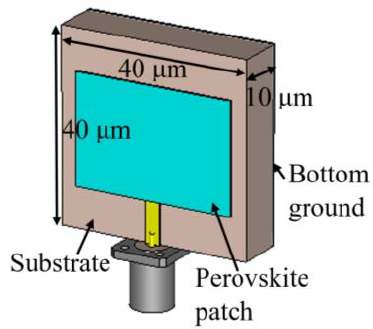
\includegraphics[width=.9\linewidth]{15}
\caption{simulated antenna design;}
\label{fig:sfig11a}
\end{subfigure}%
\begin{subfigure}{.4\textwidth}
  \centering
  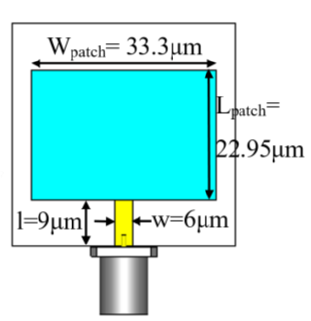
\includegraphics[width=.9\linewidth]{16}
  \caption{Perovskite patch and copper feed line in the antenna prototype.}
  \label{fig:sfigb11}
\end{subfigure}
\caption{Proposed perovskite-based THz antenna}
\label{fig:fig 11b}
\end{figure}
The reflection coefficient (\si{S_{11}}) plot of figure \ref{Fig 17} demonstrates two significant bands while taking \SI{-10 }{\deci\bel} as a reference. The band I ranges from\SI{3.6}{\THz},\SI{7.4}{\THz} and constitutes two dominant resonances at \SI{5.18}{\THz} and \SI{6.98}{\THz} respectively. The Band-II covers the range of \SI{8.25}{\THz}, \SI{10.0}{\THz} with an obvious resonant dip at \SI{8.8}{\THz}. The parametric analysis is carried out on the radiating length of the antenna and shown in figure. \ref{Fig 18}. It has been observed that with the increase in length from \SI{20.95}{\mu_m} to \SI{29.7}{\mu_m}, the resonant frequency can be tuned towards lower range.The gain and efficiency versus frequency plots are shown in figure \ref{Fig 119}, which indicates that the realized gain varies from \SI{-4.8 }{\deci\bel} in the overall operating range. The gain magnitude is above \SI{4 }{\deci\bel} in the almost complete bandwidth. Simulated results of \ref{Fig 119} also present good efficiency of 88\% at \SI{5.185}{\THz}, which is comparable to the reported graphene-based THz antenna in \cite{dashti2018graphene}. In addition, the radiation efficiency of the designed antenna could be improved by increasing the conductivity of perovskite film with the application of an external voltage.\\
\begin{figure}[hbt!]
\centering
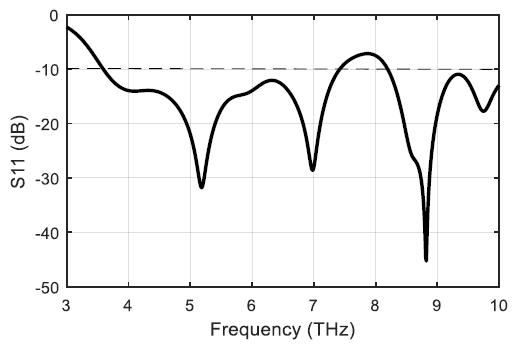
\includegraphics[width=0.5\textwidth]{17}
\caption{Simulated S11 profile of the designed perovskite-based THz antenna.}
\label{Fig 17}
\end{figure}
\begin{figure}[hbt!]
\centering
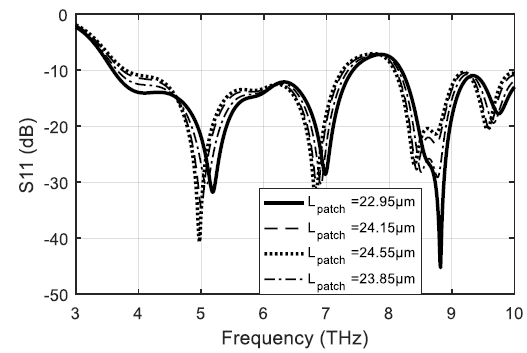
\includegraphics[width=0.5\textwidth]{18}
\caption{Parametric analysis of the radiating length of the designed perovskite based THz antenna}
\label{Fig 18}
\end{figure}
\begin{figure}[hbt!]
\centering
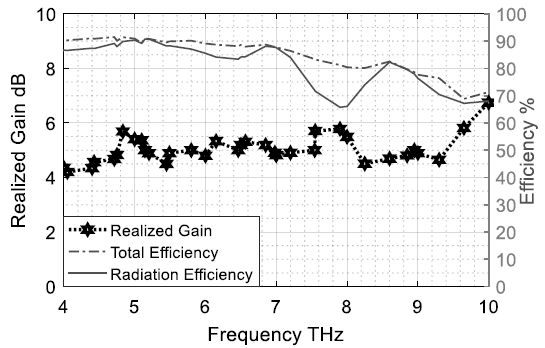
\includegraphics[width=0.5\textwidth]{19}
\caption{Realized gain and efficiency plots of the proposed perovskite based THz antenna.}
\label{Fig 119}
\end{figure}
% 
The E and H-plane radiation patterns of the designed antenna at the three major resonant frequencies are illustrated in figure.\ref{fig:fig 15}. The main lobe with \SI{4.53 }{\deci\bel} is obtained at the resonance of \SI{5.185}{\THz}, while an increase in the magnitude of main lobe gain is observed at \SI{6.985}{\THz} and \SI{8.821}{\THz} resonances. Though the radiation is not perfect broadside in the complete operating range, yet this effect is obvious when the antenna is designed to cover a wide bandwidth. The high bandwidth, reasonable gain magnitudes and high efficiency depict that the perovskite can be deployed as a radiating element in the THz patch antennas.\\
\begin{figure}[hbt!]
\begin{subfigure}{.45\textwidth}
\centering
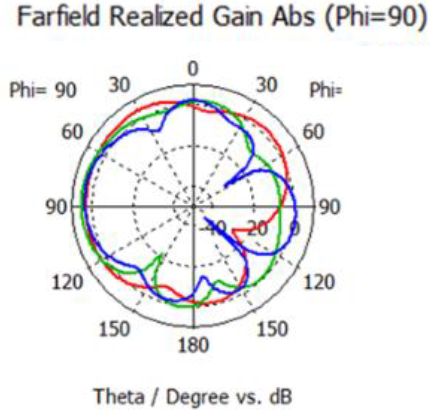
\includegraphics[width=0.9\linewidth]{20}
\caption{E-Plane}
\label{fig:sfig15a}
\end{subfigure}%
\begin{subfigure}{.45\textwidth}
  \centering
  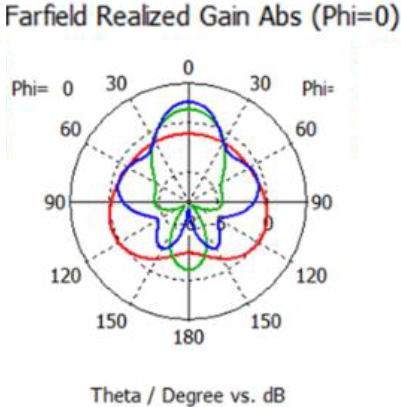
\includegraphics[width=0.9\linewidth]{21}
  \caption{H-Plane}
  \label{fig:sfigb15}
\end{subfigure}
\caption{Proposed perovskite-based THz antenna}
\label{fig:fig 15}
\end{figure}
The THz antennas are anticipated to ensure a high resolution imagining for the biomedical applications due to their short wavelength and high directivity. Novel materials have been developed for the potential deployment in modern THz systems to achieve high performance.  A newly developed perovskite material has been used for the antenna design which can replace the conventional metallic patches. The results show that the designed antenna covers two THz bands,\SI{3.6}{\THz},\SI{7.4}{\THz} and \SI{8.25}{\THz},\SI{10.0}{\THz} respectively. The realized gain of the antenna is above \SI{4 }{\deci\bel} and radiation efficiency is above 70\% in overall operating bandwidth. The antenna is regarded as a potential candidate for the future short-range THz communications.
\bibliography{bibliography.bib}
\bibliographystyle{unsrt}
\end{document}